% move all configuration stuff into includes file so we can focus on the content
\documentclass[aspectratio=169,hyperref={pdfpagelabels=false,colorlinks=true,linkcolor=white,urlcolor=blue},t]{beamer}

%%%%%%%%%%%%%%%%%%%%%%%%%%%%%%%%%%%%%%%%%%%%%%%%%%%%%%%%%%%%%%%%%%%%%%%%%%%%%%%%%%
%%%%%%%%%%%%%%%%%%%%%%%%%%%%%%%%%%%%%%%%%%%%%%%%%%%%%%%%%%%%%%%%%%%%%%%%%%%%%%%%%%
% packages
\usepackage{pict2e}
\usepackage{epic}
\usepackage{amsmath,amsfonts,amssymb}
\usepackage{units}
\usepackage{fancybox}
\usepackage[absolute,overlay]{textpos} 
\usepackage{media9} % avi2flv: "C:\Program Files\ffmpeg\bin\ffmpeg.exe" -i TuneFreqFilterbank.avi -b 600k -s 441x324 -r 15 -acodec copy TuneFreqFilterbank.flv
\usepackage{animate}
\usepackage{gensymb}
\usepackage{multirow}
\usepackage{silence}
\usepackage{tikz}
\usepackage[backend=bibtex,style=ieee]{biblatex}
\AtEveryCitekey{\iffootnote{\tiny}{}}
\addbibresource{include/references}

%%%%%%%%%%%%%%%%%%%%%%%%%%%%%%%%%%%%%%%%%%%%%%%%%%%%%%%%%%%%%%%%%%%%%%%%%%%%%%%%%%
%%%%%%%%%%%%%%%%%%%%%%%%%%%%%%%%%%%%%%%%%%%%%%%%%%%%%%%%%%%%%%%%%%%%%%%%%%%%%%%%%%
% relative paths
\graphicspath{{graph/}}


%%%%%%%%%%%%%%%%%%%%%%%%%%%%%%%%%%%%%%%%%%%%%%%%%%%%%%%%%%%%%%%%%%%%%%%%%%%%%%%%%%
%%%%%%%%%%%%%%%%%%%%%%%%%%%%%%%%%%%%%%%%%%%%%%%%%%%%%%%%%%%%%%%%%%%%%%%%%%%%%%%%%%
% units
\setlength{\unitlength}{1mm}

%%%%%%%%%%%%%%%%%%%%%%%%%%%%%%%%%%%%%%%%%%%%%%%%%%%%%%%%%%%%%%%%%%%%%%%%%%%%%%%%%%
%%%%%%%%%%%%%%%%%%%%%%%%%%%%%%%%%%%%%%%%%%%%%%%%%%%%%%%%%%%%%%%%%%%%%%%%%%%%%%%%%%
% theme & layout
\usetheme{Frankfurt}
\beamertemplatenavigationsymbolsempty
%\setbeamertemplate{frametitle}[smoothbars theme]
\setbeamertemplate{frametitle}
{
    \begin{beamercolorbox}[ht=1.8em,wd=\paperwidth]{frametitle}
        \vspace{-.1em}%
        \hspace{.2em}{\strut\insertframetitle\strut}
        
        \hspace{.2em}\small\strut\insertframesubtitle\strut
        %\hfill
        %\includegraphics[height=.8cm,keepaspectratio]{CenterMusicTechnology-solid-2lines-white-CoAtag}
        
    \end{beamercolorbox}
    \begin{textblock*}{100mm}(11.6cm,.7cm)
        \includegraphics[height=.8cm,keepaspectratio]{Logo_GTCMT_black}
    \end{textblock*}
}
\setbeamertemplate{footline}[frame number]

% set this to ensure bulletpoints without subsections
\usepackage{remreset}
\makeatletter
\@removefromreset{subsection}{section}
\makeatother
\setcounter{subsection}{1}

%---------------------------------------------------------------------------------
% appearance
\setbeamercolor{structure}{fg=gtgold}
\setbeamercovered{transparent} %invisible
\setbeamercolor{bibliography entry author}{fg=black}
\setbeamercolor*{bibliography entry title}{fg=black}
\setbeamercolor*{bibliography entry note}{fg=black}
\setbeamercolor{frametitle}{fg=black}
\setbeamercolor{title}{fg=black}

%\usepackage{pgfpages}
%\setbeameroption{show notes}
%\setbeameroption{show notes on second screen=right}
%---------------------------------------------------------------------------------
% fontsize
\let\Tiny=\tiny

%%%%%%%%%%%%%%%%%%%%%%%%%%%%%%%%%%%%%%%%%%%%%%%%%%%%%%%%%%%%%%%%%%%%%%%%%%%%%%%%%%
%%%%%%%%%%%%%%%%%%%%%%%%%%%%%%%%%%%%%%%%%%%%%%%%%%%%%%%%%%%%%%%%%%%%%%%%%%%%%%%%%%
% warnings
\pdfsuppresswarningpagegroup=1
\WarningFilter{biblatex}{Patching footnotes failed}
\WarningFilter{latexfont}{Font shape}
\WarningFilter{latexfont}{Some font shapes}
\WarningFilter{gensymb}{Not defining}


%%%%%%%%%%%%%%%%%%%%%%%%%%%%%%%%%%%%%%%%%%%%%%%%%%%%%%%%%%%%%%%%%%%%%%%%%%%%%%%%%%
%%%%%%%%%%%%%%%%%%%%%%%%%%%%%%%%%%%%%%%%%%%%%%%%%%%%%%%%%%%%%%%%%%%%%%%%%%%%%%%%%%
% theme & layout
\usetheme{Frankfurt}
\useinnertheme{rectangles}


%%%%%%%%%%%%%%%%%%%%%%%%%%%%%%%%%%%%%%%%%%%%%%%%%%%%%%%%%%%%%%%%%%%%%%%%%%%%%%%%%%
\setbeamertemplate{frametitle}[default][colsep=-4bp,rounded=false,shadow=false]
\setbeamertemplate{frametitle}
{%
    \nointerlineskip%
    %\vskip-0.5ex
    \begin{beamercolorbox}[wd=\paperwidth,ht=3.5ex,dp=0.6ex]{frametitle}
        \hspace*{1.3ex}\insertframetitle%
        
        \hspace*{1.3ex}\small\insertframesubtitle%
    \end{beamercolorbox}%
    \begin{textblock*}{100mm}(11.6cm,.57cm)
        
\includegraphics[height=.8cm,keepaspectratio]{graph/Logo_GTCMT_white}
    \end{textblock*}
}


%%%%%%%%%%%%%%%%%%%%%%%%%%%%%%%%%%%%%%%%%%%%%%%%%%%%%%%%%%%%%%%%%%%%%%%%%%%%%%%%%%
\setbeamertemplate{title page}[default][colsep=-4bp,rounded=false,shadow=false]
\setbeamertemplate{title page}
{
    \begin{textblock*}{100mm}(15cm,.51cm)
            \href{https://github.com/alexanderlerch/ACA-Slides/blob/2nd_edition/\jobname.pdf}{\includegraphics[height=.5cm,keepaspectratio]{graph/Logo_github}}\hspace*{2ex}
    \end{textblock*}
    \vskip-10ex
    \begin{beamercolorbox}[wd=\paperwidth,ht=.7\paperheight,dp=0.6ex]{frametitle} %35ex
        %\begin{flushright}
            %\href{http://www.gtcmt.gatech.edu}{\includegraphics[height=.8cm,keepaspectratio]{graph/Logo_GTCMT_black}}\hspace*{2ex}
        %\end{flushright}
        
        \hspace*{1.8ex}\LARGE\inserttitle%
        
        \vspace*{.5ex}
        
        \hspace*{1.3ex}\small\insertsubtitle%
        
        \vspace*{.5ex}
    \end{beamercolorbox}%
    \nointerlineskip%
    \begin{beamercolorbox}[wd=\paperwidth,ht=.4\paperheight,dp=0.6ex]{page number in head/foot}
        %\vspace*{-.5ex}
        \hspace*{1.7ex}\small\insertauthor%
        
        %\hspace*{1.7ex}\small }%
        
        \vspace*{10ex}
        
        \begin{flushright}
            \href{http://www.gtcmt.gatech.edu}{\includegraphics[height=.8cm,keepaspectratio]{graph/Logo_GTCMT_black}}\hspace*{2ex}
        \end{flushright}
    \end{beamercolorbox}%
}


%%%%%%%%%%%%%%%%%%%%%%%%%%%%%%%%%%%%%%%%%%%%%%%%%%%%%%%%%%%%%%%%%%%%%%%%%%%%%%%%%%
%\makeatother
\setbeamertemplate{footline}
{
  \leavevmode%
  \hbox{%
  \begin{beamercolorbox}[wd=.5\paperwidth,ht=2.25ex,dp=1ex,left,leftskip=1ex]{page number in head/foot}%
    \insertsubtitle
  \end{beamercolorbox}%
  \begin{beamercolorbox}[wd=.5\paperwidth,ht=2.25ex,dp=1ex,right,rightskip=1ex]{page number in head/foot}%
    \hfill
    \insertframenumber{} / \inserttotalframenumber
  \end{beamercolorbox}}%
  \vskip0pt%
}
%\makeatletter


%%%%%%%%%%%%%%%%%%%%%%%%%%%%%%%%%%%%%%%%%%%%%%%%%%%%%%%%%%%%%%%%%%%%%%%%%%%%%%%%%%
\beamertemplatenavigationsymbolsempty
\setbeamertemplate{navigation symbols}{}
\setbeamertemplate{blocks}[default]%[rounded=false,shadow=false]
\setbeamertemplate{itemize item}[square]
\setbeamertemplate{itemize subitem}[circle]
\setbeamertemplate{itemize subsubitem}[triangle]
\setbeamertemplate{enumerate item}[square]
\setbeamertemplate{enumerate subitem}[circle]
\setbeamertemplate{enumerate subsubitem}[circle]


%%%%%%%%%%%%%%%%%%%%%%%%%%%%%%%%%%%%%%%%%%%%%%%%%%%%%%%%%%%%%%%%%%%%%%%%%%%%%%%%%%
% colors
\setbeamercolor{structure}{fg=darkgray}
\setbeamercovered{transparent} %invisible
\setbeamercolor{bibliography entry author}{fg=black}
\setbeamercolor*{bibliography entry title}{fg=black}
\setbeamercolor*{bibliography entry note}{fg=black}
\setbeamercolor{frametitle}{fg=black}
\setbeamercolor{title}{fg=white}
\setbeamercolor{subtitle}{fg=white}
\setbeamercolor{frametitle}{fg=white}
\setbeamercolor{framesubtitle}{fg=white}
\setbeamercolor{mini frame}{fg=white, bg=black}
\setbeamercolor{section in head/foot}{fg=white, bg=darkgray}
\setbeamercolor{page number in head/foot}{fg=black, bg=lightblue}
\setbeamercolor{item projected}{fg=white, bg=black}

%---------------------------------------------------------------------------------
%%%%%%%%%%%%%%%%%%%%%%%%%%%%%%%%%%%%%%%%%%%%%%%%%%%%%%%%%%%%%%%%%%%%%%%%%%%%%%%%%%
%%%%%%%%%%%%%%%%%%%%%%%%%%%%%%%%%%%%%%%%%%%%%%%%%%%%%%%%%%%%%%%%%%%%%%%%%%%%%%%%%%
% title information
\title[]{Introduction to \textbf{Audio Content Analysis}}   
\author[alexander lerch]{alexander lerch} 
%\institute{~}
%\date[Alexander Lerch]{}
%\titlegraphic{\vspace{-16mm}\includegraphics[width=\textwidth,height=3cm]{title}}

%%%%%%%%%%%%%%%%%%%%%%%%%%%%%%%%%%%%%%%%%%%%%%%%%%%%%%%%%%%%%%%%%%%%%%%%%%%%%%%%%%
%%%%%%%%%%%%%%%%%%%%%%%%%%%%%%%%%%%%%%%%%%%%%%%%%%%%%%%%%%%%%%%%%%%%%%%%%%%%%%%%%%
% colors
\definecolor{gtgold}{HTML}{E0AA0F} %{rgb}{0.88,0.66,1,0.06} [234, 170, 0]/256
\definecolor{darkgray}{rgb}{.1, .1, .25}
\definecolor{lightblue}{rgb}{.1, 0.75, 1}
\definecolor{highlight}{rgb}{0, 0, 1} %_less!40

%%%%%%%%%%%%%%%%%%%%%%%%%%%%%%%%%%%%%%%%%%%%%%%%%%%%%%%%%%%%%%%%%%%%%%%%%%%%%%%%%%
%%%%%%%%%%%%%%%%%%%%%%%%%%%%%%%%%%%%%%%%%%%%%%%%%%%%%%%%%%%%%%%%%%%%%%%%%%%%%%%%%%
% relative paths
\graphicspath{{../ACA-Plots/graph/}}


%%%%%%%%%%%%%%%%%%%%%%%%%%%%%%%%%%%%%%%%%%%%%%%%%%%%%%%%%%%%%%%%%%%%%%%%%%%%%%%%%%
%%%%%%%%%%%%%%%%%%%%%%%%%%%%%%%%%%%%%%%%%%%%%%%%%%%%%%%%%%%%%%%%%%%%%%%%%%%%%%%%%%
% units
\setlength{\unitlength}{1mm}

%%%%%%%%%%%%%%%%%%%%%%%%%%%%%%%%%%%%%%%%%%%%%%%%%%%%%%%%%%%%%%%%%%%%%%%%%%%%%%%%%%
%%%%%%%%%%%%%%%%%%%%%%%%%%%%%%%%%%%%%%%%%%%%%%%%%%%%%%%%%%%%%%%%%%%%%%%%%%%%%%%%%%
% math
\DeclareMathOperator*{\argmax}{argmax}
\DeclareMathOperator*{\argmin}{argmin}
\DeclareMathOperator*{\atan}{atan}
\DeclareMathOperator*{\arcsinh}{arcsinh}
\DeclareMathOperator*{\sign}{sign}
\DeclareMathOperator*{\tcdf}{tcdf}
\DeclareMathOperator*{\si}{sinc}
\DeclareMathOperator*{\princarg}{princarg}
\DeclareMathOperator*{\arccosh}{arccosh}
\DeclareMathOperator*{\hwr}{HWR}
\DeclareMathOperator*{\flip}{flip}
\DeclareMathOperator*{\sinc}{sinc}
\DeclareMathOperator*{\floor}{floor}
\newcommand{\e}{{e}}
\newcommand{\jom}{\mathrm{j}\omega}
\newcommand{\jOm}{\mathrm{j}\Omega}
\newcommand   {\mat}[1]    		{\boldsymbol{\uppercase{#1}}}		%bold
\renewcommand {\vec}[1]    		{\boldsymbol{\lowercase{#1}}}		%bold

%%%%%%%%%%%%%%%%%%%%%%%%%%%%%%%%%%%%%%%%%%%%%%%%%%%%%%%%%%%%%%%%%%%%%%%%%%%%%%%%%%
%%%%%%%%%%%%%%%%%%%%%%%%%%%%%%%%%%%%%%%%%%%%%%%%%%%%%%%%%%%%%%%%%%%%%%%%%%%%%%%%%%
% media9
\newcommand{\includeaudio}[1]{
\href{run:audio/#1.mp3}{
\includegraphics[width=5mm, height=5mm]{graph/SpeakerIcon}}}

\newcommand{\includeanimation}[4]{{\begin{center}
                        \animategraphics[autoplay,loop,scale=.7]{#4}{animation/#1-}{#2}{#3}        
                        \end{center}
                        \addreference{matlab source: \href{https://github.com/alexanderlerch/ACA-Plots/blob/master/matlab/animate#1.m}{matlab/animate#1.m}}}
                        \inserticon{video}}
                        
%%%%%%%%%%%%%%%%%%%%%%%%%%%%%%%%%%%%%%%%%%%%%%%%%%%%%%%%%%%%%%%%%%%%%%%%%%%%%%%%%%
%%%%%%%%%%%%%%%%%%%%%%%%%%%%%%%%%%%%%%%%%%%%%%%%%%%%%%%%%%%%%%%%%%%%%%%%%%%%%%%%%%
% other commands
\newcommand{\question}[1]{%\vspace{-4mm}
                          \setbeamercovered{invisible}
                          \begin{columns}[T]
                            \column{.9\textwidth}
                                \textbf{#1}
                            \column{.1\textwidth}
                                \vspace{-8mm}
                                \begin{flushright}
                                     
\includegraphics[width=.9\columnwidth]{graph/question_mark}
                                \end{flushright}
                                \vspace{6mm}
                          \end{columns}\pause\vspace{-12mm}}

\newcommand{\toremember}[1]{
                        \inserticon{lightbulb}
                        }

\newcommand{\matlabexercise}[1]{%\vspace{-4mm}
                          \setbeamercovered{invisible}
                          \begin{columns}[T]
                            \column{.8\textwidth}
                                \textbf{matlab exercise}: #1
                            \column{.2\textwidth}
                                \begin{flushright}
                                     \includegraphics[scale=.5]{graph/logo_matlab}
                                \end{flushright}
                                %\vspace{6mm}
                          \end{columns}}

\newcommand{\addreference}[1]{  
                  
                    \begin{textblock*}{\baselineskip }(.98\paperwidth,.5\textheight) %(1.15\textwidth,.4\textheight)
                         \begin{minipage}[b][.5\paperheight][b]{1cm}%
                            \vfill%
                             \rotatebox{90}{\tiny {#1}}
                        \end{minipage}
                   \end{textblock*}
                    }
                    
\newcommand{\figwithmatlab}[1]{
                    \begin{figure}
                        \centering
                        \includegraphics[scale=.7]{#1}
                        %\label{fig:#1}
                    \end{figure}
                    
                    \addreference{matlab source: \href{https://github.com/alexanderlerch/ACA-Plots/blob/main/matlab/plot#1.m}{plot#1.m}}}
\newcommand{\figwithref}[2]{
                    \begin{figure}
                        \centering
                        \includegraphics[scale=.7]{#1}
                        \label{fig:#1}
                    \end{figure}
                    
                    \addreference{#2}}  
                                    
\newcommand{\inserticon}[1]{
                    \begin{textblock*}{100mm}(14.5cm,7.5cm)
                        \includegraphics[height=.8cm,keepaspectratio]{graph/#1}
                    \end{textblock*}}            

%%%%%%%%%%%%%%%%%%%%%%%%%%%%%%%%%%%%%%%%%%%%%%%%%%%%%%%%%%%%%%%%%%%%%%%%%%%%%%%%%%
%%%%%%%%%%%%%%%%%%%%%%%%%%%%%%%%%%%%%%%%%%%%%%%%%%%%%%%%%%%%%%%%%%%%%%%%%%%%%%%%%%
% counters
\newcounter{i}
\newcounter{j}
\newcounter{iXOffset}
\newcounter{iYOffset}
\newcounter{iXBlockSize}
\newcounter{iYBlockSize}
\newcounter{iYBlockSizeDiv2}
\newcounter{iXBlockSizeDiv2}
\newcounter{iDistance}




\subtitle{Module 15: Music Performance Analysis}

%%%%%%%%%%%%%%%%%%%%%%%%%%%%%%%%%%%%%%%%%%%%%%%%%%%%%%%%%%%%%%%%%%%%%%%%%%%%
\begin{document}
    % generate title page
	{
\setbeamertemplate{headline}{} 
\setbeamertemplate{footline}{} 
\begin{frame}
    \titlepage
    %\vspace{-5mm}
\end{frame}
}
\addtocounter{framenumber}{-1}


    \section[overview]{lecture overview}
        \begin{frame}{introduction}{overview}
            \begin{block}{corresponding textbook section}
                    %\href{http://ieeexplore.ieee.org/xpl/articleDetails.jsp?arnumber=6331125}{Chapter 8: Musical Genre, Similarity, and Mood} (pp.~158--161)
                    chapter~15
            \end{block}

            \begin{itemize}
                \item   \textbf{lecture content}
                    \begin{itemize}
                        \item   musical communication
                        \item   music performance
                        \item   music performance analysis
                    \end{itemize}
                \bigskip
                \item<2->   \textbf{learning objectives}
                    \begin{itemize}
                        \item   give examples for score-inherent and performance-inherent musical characteristics
                        \item   describe typical challenges in music performance analysis
                    \end{itemize}
            \end{itemize}
            \inserticon{directions}
        \end{frame}

    \section{music performance}
        \begin{frame}{music performance}{introduction}
            \vspace{-5mm}
            \begin{columns}
            \column{0.4\linewidth}
            \begin{itemize}
                \item	music exists only with performance
                \item   performance realizes acoustic rendition of musical ideas 
                \item   each rendition is unique
                \item   score information is interpreted, modified, added to, or dismissed
                \item   adds ``expressivity''
            \end{itemize}
            \column{0.6\linewidth}
            
                \begin{figure}
                   \scalebox{.5}{\begin{footnotesize}
\setcounter{iXOffset}{0}
\setcounter{iYOffset}{4}
\setcounter{iXBlockSize}{24}
\setcounter{iYBlockSize}{8}
\setcounter{iDistance}{8}
\setcounter{iYBlockSizeDiv2}{4}
\begin{picture}(152,24)

	\put(\value{iXOffset}, \value{iYOffset})
		{\framebox(\value{iXBlockSize}, \value{iYBlockSize}) {{\shortstack[c]{Composition}}}}
	\addtocounter{iXOffset}{\value{iXBlockSize}}
	\addtocounter{iYOffset}{\value{iYBlockSizeDiv2}}
	\put(\value{iXOffset}, \value{iYOffset})
		{\vector(1,0){\value{iDistance}}}
	\addtocounter{iYOffset}{-\value{iYBlockSizeDiv2}}
	\addtocounter{iXOffset}{\value{iDistance}}
	
	\put(\value{iXOffset}, \value{iYOffset})
		{\framebox(\value{iXBlockSize}, \value{iYBlockSize}) {{\shortstack[c]{Performance}}}}
	\addtocounter{iXOffset}{\value{iXBlockSize}}
	\addtocounter{iYOffset}{\value{iYBlockSizeDiv2}}
	\put(\value{iXOffset}, \value{iYOffset})
		{\vector(1,0){\value{iDistance}}}
	\addtocounter{iYOffset}{-\value{iYBlockSizeDiv2}}
	\addtocounter{iXOffset}{\value{iDistance}}
	
	\put(\value{iXOffset}, \value{iYOffset})
		{\framebox(\value{iXBlockSize}, \value{iYBlockSize}) {{\shortstack[c]{Production}}}}
	\addtocounter{iXOffset}{\value{iXBlockSize}}
	\addtocounter{iYOffset}{\value{iYBlockSizeDiv2}}
	\put(\value{iXOffset}, \value{iYOffset})
		{\vector(1,0){\value{iDistance}}}
	\addtocounter{iYOffset}{-\value{iYBlockSizeDiv2}}
	\addtocounter{iXOffset}{\value{iDistance}}
	
	\put(\value{iXOffset}, \value{iYOffset})
		{\framebox(\value{iXBlockSize}, \value{iYBlockSize}) {{\shortstack[c]{Reproduction}}}}
	\addtocounter{iXOffset}{\value{iXBlockSize}}
	\addtocounter{iYOffset}{\value{iYBlockSizeDiv2}}
	\put(\value{iXOffset}, \value{iYOffset})
		{\vector(1,0){\value{iDistance}}}
	\addtocounter{iYOffset}{-\value{iYBlockSizeDiv2}}
	\addtocounter{iXOffset}{\value{iDistance}}
	
	\put(\value{iXOffset}, \value{iYOffset})
		{\framebox(\value{iXBlockSize}, \value{iYBlockSize}) {{\shortstack[c]{Reception}}}}
	\addtocounter{iXOffset}{\value{iXBlockSize}}
	\addtocounter{iYOffset}{\value{iYBlockSizeDiv2}}

    % additional stuff
    \setcounter{iXOffset}{60}
    \setcounter{iYOffset}{0}
	\put(\value{iXOffset}, \value{iYOffset})
		{\dashbox{2}(64, 16) {~}}
        
	\addtocounter{iXOffset}{\value{iXBlockSize}}
	\addtocounter{iXOffset}{\value{iDistance}}
	\addtocounter{iYOffset}{\value{iYBlockSize}}
	\addtocounter{iDistance}{\value{iYBlockSizeDiv2}}
	\addtocounter{iYOffset}{\value{iDistance}}
	\put(\value{iXOffset}, \value{iYOffset})
		{\vector(0,-1){\value{iDistance}}}
        
	\addtocounter{iXOffset}{-14}
	\addtocounter{iYOffset}{2}
	\put(\value{iXOffset}, \value{iYOffset})
		{\text{\shortstack[c]{Recording to Analyze}}}
        
	%%feedback					
	%\addtocounter{iXOffset}{-11}
	%\addtocounter{iYOffset}{-8}
	%\put(\value{iXOffset}, \value{iYOffset})
		%{\line(-1,0){21}}
	%\put(\value{iXOffset}, \value{iYOffset})
		%{\line(0,1){3}}
	%\addtocounter{iXOffset}{-21}
	%\put(\value{iXOffset}, \value{iYOffset})
		%{\vector(0,1){3}}
	%\addtocounter{iXOffset}{32}
	%\addtocounter{iYOffset}{8}
	
	%\addtocounter{iYOffset}{-\value{iYBlockSizeDiv2}}
	%\addtocounter{iXOffset}{\value{iDistance}}
	%
	%\put(\value{iXOffset}, \value{iYOffset})
		%{\dashbox(\value{iXBlockSize}, \value{iYBlockSize}) {{\shortstack[c]{Production}}}}
	%\addtocounter{iXOffset}{\value{iXBlockSize}}
	%\addtocounter{iYOffset}{\value{iYBlockSizeDiv2}}
	%\put(\value{iXOffset}, \value{iYOffset})
		%{\vector(1,0){\value{iDistance}}}
%
	%%feedback					
	%\addtocounter{iXOffset}{-11}
	%\addtocounter{iYOffset}{-8}
	%\put(\value{iXOffset}, \value{iYOffset})
		%{\line(-1,0){21}}
	%\put(\value{iXOffset}, \value{iYOffset})
		%{\line(0,1){3}}
	%\addtocounter{iXOffset}{-21}
	%\put(\value{iXOffset}, \value{iYOffset})
		%{\vector(0,1){3}}
	%\addtocounter{iXOffset}{32}
	%\addtocounter{iYOffset}{8}
	%
	%\addtocounter{iYOffset}{-\value{iYBlockSizeDiv2}}
	%\addtocounter{iXOffset}{\value{iDistance}}
	%
	%\put(\value{iXOffset}, \value{iYOffset})
		%{\framebox(\value{iXBlockSize}, \value{iYBlockSize}) {{\shortstack[c]{(Acoustic)\\ Channel}}}}
	%\addtocounter{iXOffset}{\value{iXBlockSize}}
	%\addtocounter{iYOffset}{\value{iYBlockSizeDiv2}}
%%	\put(\value{iXOffset}, \value{iYOffset})
%%		{\vector(1,0){\value{iDistance}}}
		%
	%%feedback
	%\addtocounter{iXOffset}{-10}
	%\addtocounter{iYOffset}{-9}
	%\put(\value{iXOffset}, \value{iYOffset})
		%{\line(-1,0){46}}
	%\put(\value{iXOffset}, \value{iYOffset})
		%{\line(0,1){4}}
	%\addtocounter{iXOffset}{-46}
	%\put(\value{iXOffset}, \value{iYOffset})
		%{\vector(0,1){4}}
	%\addtocounter{iXOffset}{46}
	%%\addtocounter{iXOffset}{10}
	%\addtocounter{iYOffset}{9}
		%
	%\addtocounter{iYOffset}{\value{iYBlockSizeDiv2}}
	%
	%\put(\value{iXOffset}, \value{iYOffset})
		%{\vector(0,1){\value{iDistance}}}
%
	%\addtocounter{iXOffset}{-5}
%
				
\end{picture}
\end{footnotesize}
	}
                \end{figure}
            \end{columns}
            
            \bigskip
            \includeaudio{performance_example1}\hspace{5mm}  \includeaudio{performance_example2}

            \vspace{-30mm}
            \flushright{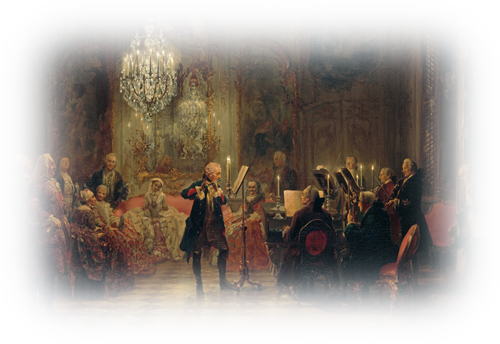
\includegraphics[scale=.7]{graph/performance}}
            %\begin{flushright}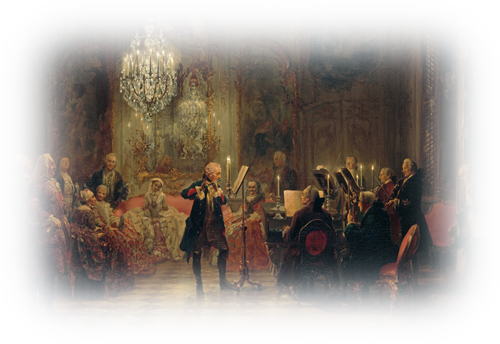
\includegraphics{graph/performance}\end{flushright}
        \end{frame}
        \begin{frame}{music performance}{parameters}
            \begin{table}
            \begin{tabular}{lll}
                \textbf{category}   & \textbf{score representation/idea} & \textbf{performance} \\
                tempo/timing        & explicitly defined rhythmic content&  tempo, micro-timing\\
                dynamics            &basic dynamics instructions            & accents,...\\
                pitch               & explicitely defined pitches           & vibrato, intonation,...\\
                timbre              & implicit definitions (instruments, ..) & playing techniques
            \end{tabular}
            \end{table}
            
        \end{frame}
   
    \section[performance analysis]{music performance analysis}
        \begin{frame}{music performance analysis}{goals}
            by analyzing the music performance, we learn about
            \bigskip

            \begin{itemize}
                \item	the \textbf{performance}: 
                    \begin{itemize}
                        \item   general performance characteristics
                        \item   notable stylistic differences (over time, between artists, ...)
                    \end{itemize}
                \item	the \textbf{performer}: 
                    \begin{itemize}
                        \item   mapping of intent and projected emotion to measurable parameters
                    \end{itemize}
                \item	the \textbf{listener}: 
                    \begin{itemize}
                        \item   what is perceived as (appropriate level of) expressiveness
                        \item   how can different performance parameters impact the listener
                        \item   how is aesthetic perception shaped by performance parameters
                    \end{itemize}
            \end{itemize}

            \begin{textblock*}{100mm}(12.5cm,1.5cm)
                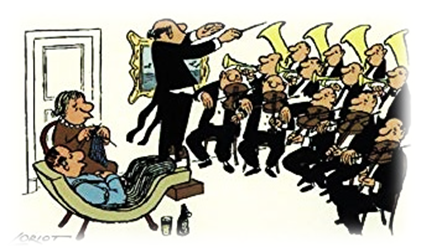
\includegraphics[scale=.5,keepaspectratio]{graph/life_concert}
            \end{textblock*}
 
            %\vspace{-20mm}
            %\flushright{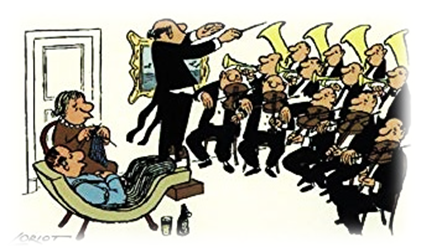
\includegraphics[scale=.5]{graph/life_concert}}
        \end{frame}
            
        \begin{frame}{performance analysis}{insights 1/3}
            \vspace{-5mm}
            \begin{columns}
            \column{0.4\linewidth}
            \begin{itemize}
                \item close relation between \textbf{tempo/dynamics and structure}:
                    \begin{itemize}
                        \item	ritardandi at phrase boundaries
                        \item   tempo changes at structural boundaries 
                        \item   repetitions very similar
                    \end{itemize}
                \item   performance sounds unnatural without these general trends
                \item   no clear relation to timbre
            \end{itemize}
            \column{0.6\linewidth}
            
                \begin{figure}
                   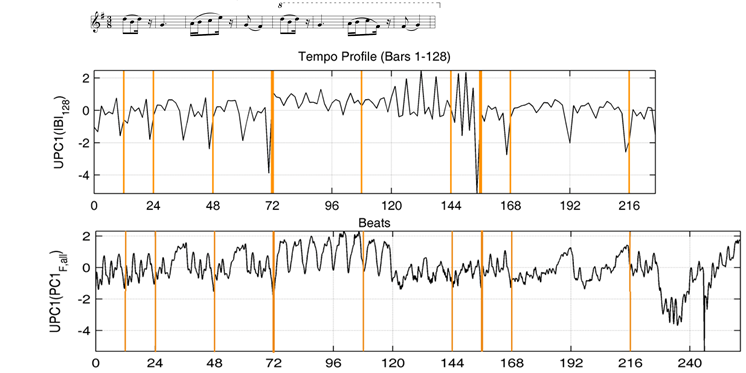
\includegraphics[width=\columnwidth]{graph/tempo_loudness}
                \end{figure}
            \end{columns}
       \end{frame}
        \begin{frame}{performance analysis}{insights 2/3}
            \begin{itemize}
                \item perceptual relevance of “expressive” performance characteristics:
                    \begin{itemize}
                        \item	dynamics highest impact on ratings of emotional expression
                        \item   expressive timing best predicts ratings of musical tension
                        \item   sharpened intonation at phrase climax contributes to perceived excitement
                    \end{itemize}
                \item   measured $\neq$ perceived
                    \begin{itemize}
                        \item	e.g., measurable difference between “normative” and ``expressive'' performance does not necessarily lead to perception of expressivity 
                        \item   e.g., no correlation between measured and perceived vibrato onsets
                    \end{itemize}
            \end{itemize}
       \end{frame}
        \begin{frame}{performance analysis}{insights 3/3}
            \vspace{-5mm}
            \begin{columns}
            \column{0.6\linewidth}
            \begin{itemize}
                \item Humans rate performances regularly (schools, auditions, competitions) but specific criteria are often badly defined
                \item use cases
                    \begin{itemize}
                        \item	music education
                        \item computer-assisted practice
                        \item pre-screening of candidates for music programs
                        \item provide insights into \textbf{technical and aesthetical descriptors} of human judgments
                    \end{itemize}
                \item   most models still lack generalizability and reliability beyond simple note matching

            \end{itemize}
            \column{0.4\linewidth}
            
                \begin{figure}
                   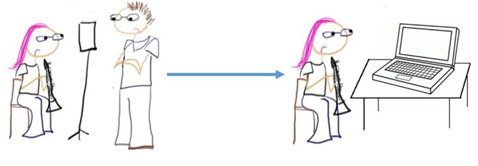
\includegraphics[width=\columnwidth]{graph/performance_assessment}
                \end{figure}
            \end{columns}
       \end{frame}
        
    \section{challenges}
  
        \begin{frame}{music performance analysis}{challenges}
            \begin{itemize}
                \item   \textbf{observations}
                    \begin{itemize}
                        \item   style dependent, lacking research beyond western classical music
                        \item   data is manually annotated in most cases
                        \item   most research 
                            \begin{itemize}
                                \item   focused on piano and voice 
                                \item   descriptive and explorative
                            \end{itemize}
                    \end{itemize}
                    \bigskip
                    \begin{enumerate}
                        \item   datasets small, not general
                            \begin{itemize}
                                \item automatic tools not reliable enough?
                                \item   generality: instrument specific, performers, listeners
                            \end{itemize}
                        \item   unknown mapping of performance parameters to perception
                            \begin{itemize}
                                \item   isolation of parameter meaning tricky
                                \item   hard to define expressivity, hard to control variables
                            \end{itemize}
                    \end{enumerate}
            \end{itemize}

        \end{frame}
        \begin{frame}{music performance analysis}{opportunities}
            \begin{itemize}
                \item   understanding why current MIR systems are of limited use to music psychologists and performance researchers
                    \begin{itemize}
                        \item   wrong measures of success?
                        \item   miscommunication of system capabilities?
                    \end{itemize}
                \bigskip
                \item   score-based and performance-based information should be disentangled
                    \begin{itemize}
                        \item   lack of separation of core musical ideas and performance characteristics impedes differentiation of relevant and irrelevant information (example: music emotion recognition)
                    \end{itemize}
                \bigskip
                \item   cross-disciplinary approaches and methodologies can help
                    \begin{itemize}
                        \item   enabling larger scale perceptual studies with music data
                        \item   interpretability of data 
                            \begin{itemize}
                                \item   better understanding of music and its perception 
                                \item   better systems for music analysis and music generation
                            \end{itemize}
                    \end{itemize}
            \end{itemize}

        \end{frame}
    
    \section{summary}
        \begin{frame}{summary}{lecture content}
            \begin{itemize}
                \item   \textbf{performance}
                    \begin{itemize}
                        \item   all music needs to be performed
                        \item   while the general performance characteristics are clear, their analysis is less clear
                    \end{itemize}
                \bigskip
                \item   \textbf{performance analysis}
                    \begin{enumerate}
                        \item   describes and formalizes commonalities and differences of performances
                    \end{enumerate}
                \bigskip
                \item   \textbf{challenges}
                    \begin{enumerate}
                        \item   tricky to disentangle variables
                        \item   unclear impact on listeners
                        \item   hard to find reliable ground truth data
                    \end{enumerate}
            \end{itemize}
            \inserticon{summary}
        \end{frame}
\end{document}
